\documentclass{article}
\usepackage[utf8]{inputenc}
\usepackage{graphicx}
\usepackage{amsmath, amsthm, amssymb}
\usepackage{multicol}
\usepackage{svg}
\usepackage{caption}
\usepackage{vmargin}
\usepackage[hidelinks]{hyperref}
\usepackage[utf8]{inputenc}
 \usepackage{epigraph}

\theoremstyle{definition}
\newtheorem{defi}{Definition}[section]
\newtheorem{theorem}{Theorem}[section]
\newtheorem{proposition}{Proposition}[section]
\newtheorem{lemma}{Lemma}[section]

\title{Semantic Web Engineering \protect\\ Introduction}
\author{Xiaozhe Yao\footnote{https://yaonotes.org/lecture-notes}}
\date{20 Nov 2019}
\begin{document}

\maketitle
\begin{center}
    
\includegraphics[width=60px]{Semantic_Web/images/semantic-web.pdf}
\end{center}
\section{Introduction}

\say{The Web was designed as an information space, with the goal that it should be useful not only for human-human communication, but also that machines would be able to participate and help. One of the major obstacles to this has been the fact that most information on the Web is designed for human consumption, and even if it was derived from a database with well defined meanings (in at least some terms) for its columns, that the structure of the data is not evident to a robot browsing the web. Leaving aside the artificial intelligence problem of training machines to behave like people, the Semantic Web approach instead develops languages for expressing information in a machine processable form.}

It is like a global database that enables several new operations, such as Search, Personalization, Linking and Integration.

Search engines improve their capabilities in surprisingly and stunning ways, but the results are often lists of disconnected documents. Semantic web wants to find the relations between each node. It follows a different perspective,

\begin{itemize}
    \item Usage of structured and semi-structured data with standard formats.
    \item Data elements as first class citizen in the web, rather than documents.
    \item Descriptions of the semantics of data elements becomes available.
\end{itemize}

\textbf{Example of Semantic Web} The content of HTML code is organised according to presentation information, such as title, table, list, headings, etc. There exists structured data in HTML code because most web pages are generated from databases. We could therefore link the underlying structured datasets.

\subsection{Basic Technologies}

\begin{itemize}

\item \textbf{RDF (Resource Description Framework)}. RDF uses labelled graph as data models, where objects are nodes and relations are edges. It corresponds to the principle \#1: Usage of structured data and semi-structured data.

\item \textbf{URI (Uniform Resource Identifier) and IRI (Internationalized Resource Identifiers)}. They are used as web identifier. RDF relies on URI/IRI to identify data elements and relations among them. They corresponds to the principle \#2: Data Elements as first class citizen in the web.

\item \textbf{RDF Schema and OWL (Ontology Web Language)} They are used as knowledge representation languages that enable inference of implicit information in the data. To compare, RDF schema is less expressive while OWL is richer (though it depends on the dialect). RDF Schema and OWL can be used to impose upper and lower bounds to the data semantics. They corresponds to the principle \#3: Make available the data semantic description.

\end{itemize}

\subsection{Architecture and Roadmap}

The web is distributed in three pillars: Content, Location and Ownership. The semantic web inherits these three core pillars.

The three main steps to achieve the semantic web are: 
\begin{itemize}
    \item Agreement on standard syntaxes to represent data and metadata.
    \item Agreement on vocabularies to express how the data is represented and structured.
    \item Publication of large amounts of data in standard syntaxes and compliant to the agreed vocabularies.
\end{itemize}

The semantic web stack, also known as semantic web cake or semantic web layer cake, illustrates the architecture of the semantic web. It is shown as below:

\begin{center}
    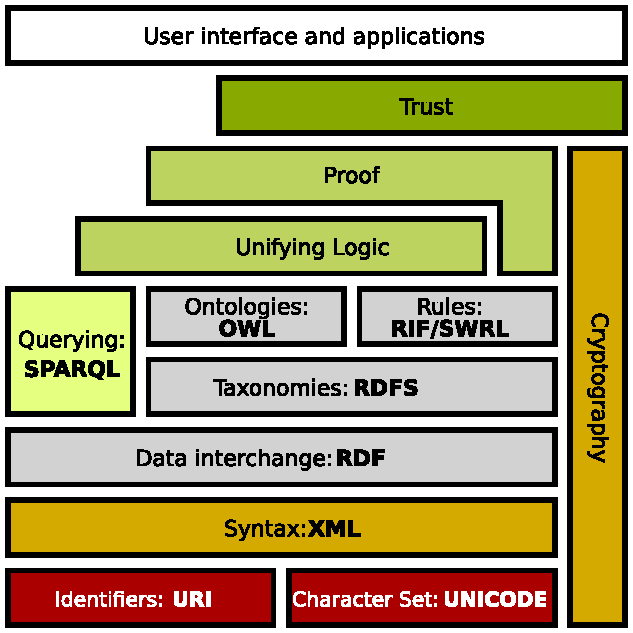
\includegraphics[width=250px]{Semantic_Web/images/Semantic_web_stack.pdf}
\end{center}

\section{URI and IRI}

URI and IRI are the building blocks that are used to identify \textit{everything}. Historically, XML played a keey role but now its roles are becoming less and less predominant. Here the \textit{everything} are the reesources thaat we want to talk about, such as things, publications, people, etc.

URI (Uniform Resource Identifier) is a string of characters that \textbf{unambiguously} identifies a particular resource. To guarantee uniformity, all URIs follow a predefined set of syntax rules, but also maintain extensibility through a separately defined hierarchical naming scheme. URLs exist in web locations, telephonee numbers, ISBN numbers, etc. Generally, everything can be attached with an URL.

Examples of URI includes:

\begin{itemize}
    \item ftp://ftp.is.co.za/rfc/rfc1808.txt
    \item mailto:John.Doe@example.com
    \item urn:oasis:names:specification:docbook:dtd:xml:4.1.2 
\end{itemize}

IRI extends URL with characters from Universal Character Set.

\subsection{URI, URL and URN}

These concepts maybe confusing. 

\begin{itemize}
    \item URL (Universal Resource Locator) is a subset of URI, which means all URLs are URIs, but not all URIs are URLs.
    \item \textbf{Main Difference between URL and URI} URLs necessarily enable the acess to a resource, that is why it is called "Locator". URIs do not neceessarily enable the access to the resource.
    \item URN (Uniform Resource Name) has been used historically to refer to both URIs under the "urn" scheme, which requires to remain globally unique and persistent even when the reource ceases to exist or becomes unavailable, and to any other URI with the properties of a name.
    \item URN uniiquely identifies a resource, while URI may uniquely identifies resources but it is not required.
    \item URN does not contain any access information.
\end{itemize}

\subsection{Anatomy of a URI}

We often use HTTP URIs to identify resources on the web. For example:

\begin{itemize}
    \item http://example.org#test $\rightarrow$ :test
    \item http://www.w3.org/1999/02/22-rdf-syntax-ns#type $\rightarrow$ rdf:type
    \item http://ddis.ch/ppl/Karl $\rightarrow$ ddis:Karl
\end{itemize}

In this example, prefixes are short stand-ins for the namespaces

\begin{itemize}
    \item rdf $\rightarrow$ http://www.w3.org/1999/02/22-rdf-syntax-ns#
    \item ddis $\rightarrow$ http://ddis.ch/people/
\end{itemize}

Prefixes are usually used to replace the namespaces, followed by ":" and the local name of the resource.

A special prefix is the default one, composed by an empty string. $\rightarrow$ http://example.org#

\end{document}